%% !TEX root = manual.tex

\section{Dragonfly}
\label{sec:tutorial:dragonfly}

\begin{figure}[h!]
\centering
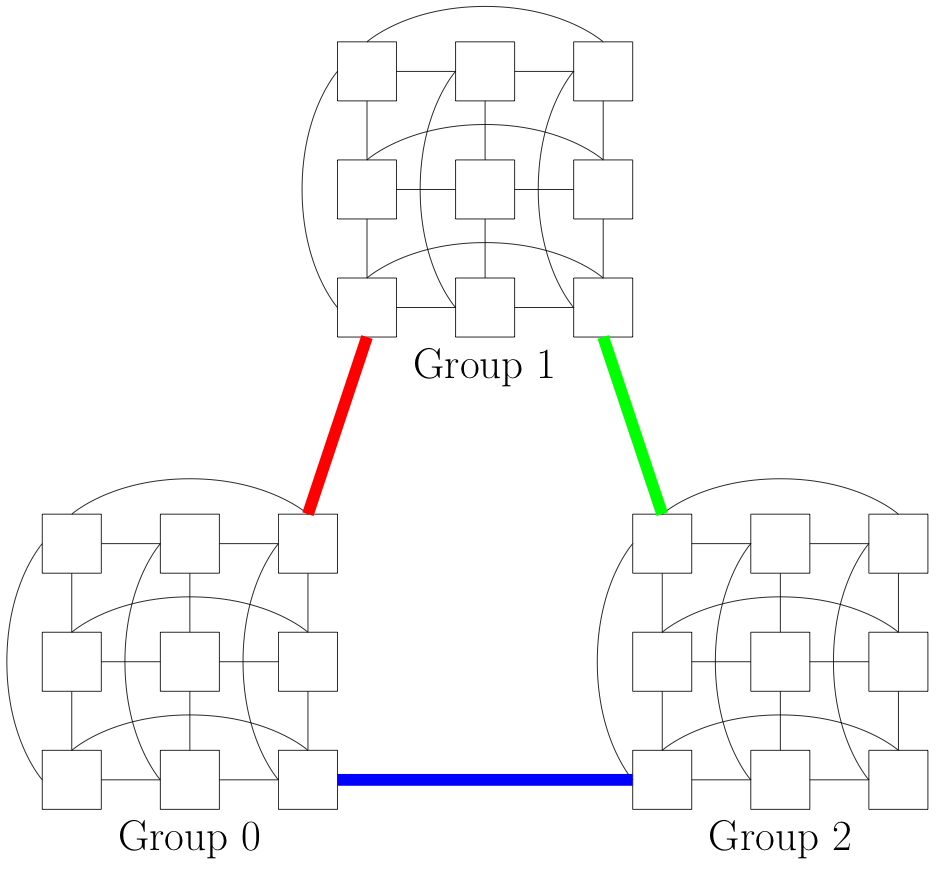
\includegraphics[width=0.7\textwidth]{figures/tikz/dragonfly/dragonfly.png}
\caption{Schematic of dragonfly with three groups showing hypercube intragroup links and high bandwidth intergroup global links}
\label{fig:topologies:dragonfly}
\end{figure}

As bandwidth per pin increases, arguments can be made that optimal topologies should be higher radix.
A 3D torus is on the low-radix extreme while a hypercube is a high-radix extreme.
Unfortunately a hypercube topology is not scalable and the radix quickly becomes too high to efficiently implement.
A dragonfly is sometimes viewed as a generalization of flattened butterfly and hypercube topologies with ``virtual'' switches of very high radix,
not dissimilar from the fat-tree implementation with many physical commodity switches composing a single virtual switch.
The dragonfly topology (Figure \ref{fig:topologies:dragonfly}) is actually quite simple. 
Small groups are connected as a generalized hypercube with full connectivity within a row or column.
Intergroup connections (global links) provide pathways for hopping between groups.
A dragonfly is usually understood through three parameters:
\begin{itemize}
\item $p$: number of nodes connected to each router
\item $a$: number of routers in a group
\item $h$: number of global links that each switch has
\end{itemize}

For simplicity, only three example global links are show for clarity in the picture.
For the Cray X630, $a = 96$, $h=10$, and $p=4$ so that each router is connected to many other ($h=10$) groups.
The caveat is that in many implementations global links are grouped together for $h=2$ or $3$ fat global links.
These demonstrate well-balanced ratios.
In general, scaling out a dragonfly should not increase the size of a group, only the number of groups.

\subsection{Allocation and indexing}
\label{subsec:dragonfly:allocatoin}

The dragonfly coordinate system is essentially the same as a 3D torus.  
The group 2D hypercube layout defines $X$ and $Y$ coordinates.
The group number defines a $Z$ or $G$ coordinate.
Thus the topology in Figure \ref{fig:topologies:dragonfly} would be specified as

\begin{ViFile}
topology.name = dragonfly
topology.geometry = 3 3 3
\end{ViFile}
for groups of size $3 \times 3$ with a total of 3 groups.
To complete the specification, the number of global links ($h$) for each router must be given
\begin{ViFile}
topology.group_connections = 10
\end{ViFile}

\subsection{Routing}
\label{subsec:dragonfly:routing}

It is important to understand the distinction between link bandwidth, channel bandwidth, and pin bandwidth.
All topologies have the same pin bandwidth and channel bandwidth (assuming they use the same technology).
Each router in a topology is constrained to have the same number of channels (called radix, usually about $k=64$).
The number of channels per link changes dramatically from topology to topology.
Low radix topologies like 3D torus can allocate more channels per link, 
giving higher bandwidth between adjacent routers.
Dragonfly is higher radix, having many more connections but having lower bandwidth between adjacent routers.
While minimal routing is often sufficient on torus topologies because of the high link bandwidth,
dragonfly will exhibit very poor performance with minimal routing.
To effectively utilize all the available bandwidth, packets should have a high amount of path diversity.
Packets sent between two routers should take as many different paths as possible to maximize the effective bandwidth point-to-point.

\begin{figure}[h!]
\centering
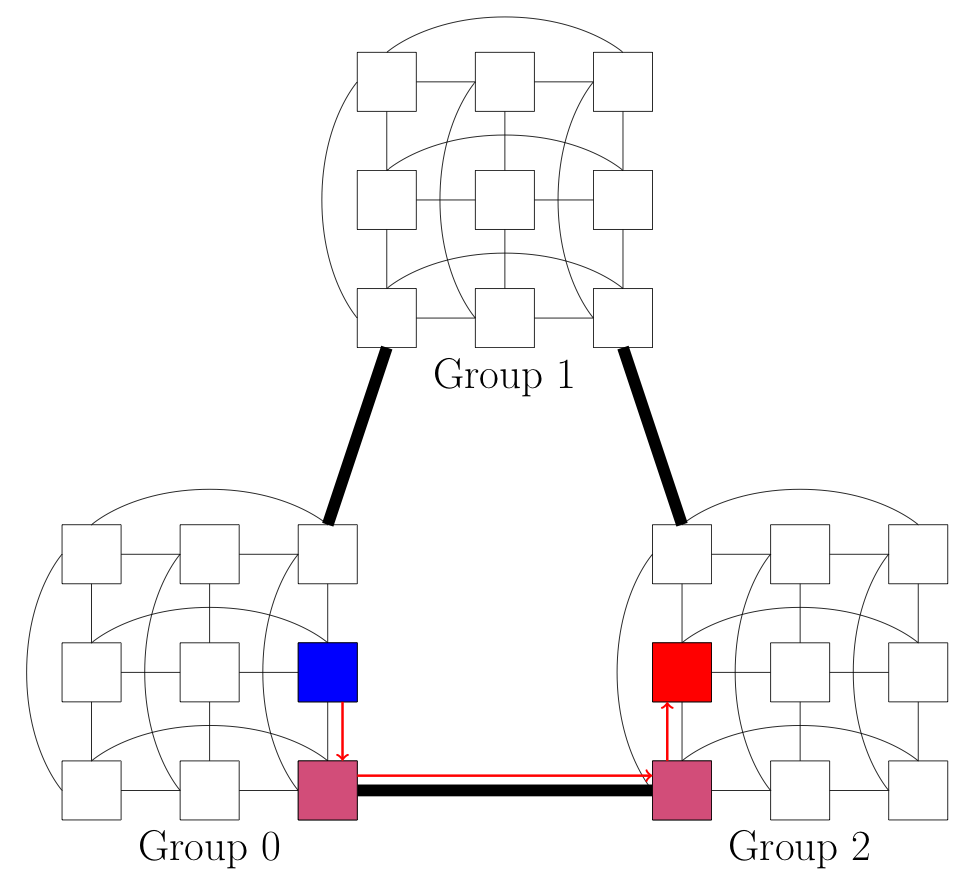
\includegraphics[width=0.7\textwidth]{figures/tikz/dragonfly/dflyminroute.png}
\caption{Schematic of dragonfly showing minimal route. Traveling between groups requires routing to the correct global link, hopping the global link, then routing within a group to the correct final node.}
\label{fig:topologies:dflyminroute}
\end{figure}

Minimal routing itself has a few complications (Figure \ref{fig:topologies:dflyminroute}).  
Each router only has a few global links.  
Thus, traveling from e.g. the blue router at X=3,Y=2,G=0 to the red router at X=1,Y=2,G=2, there is no direct link between the routers.
Furthermore, there is no direct link between Groups 0 and 2.
Thus packets must route through the purple intermediate nodes.
First, the packet hops to X=3,Y=3, G=0.  
This router has a global link to Group 2, allowing the packet to hop to the next intermediate router at X=1, Y=3, G=2.
Finally, the minimal route completes by hopping within Group 2 to the final destination.

\begin{figure}[h!]
\centering
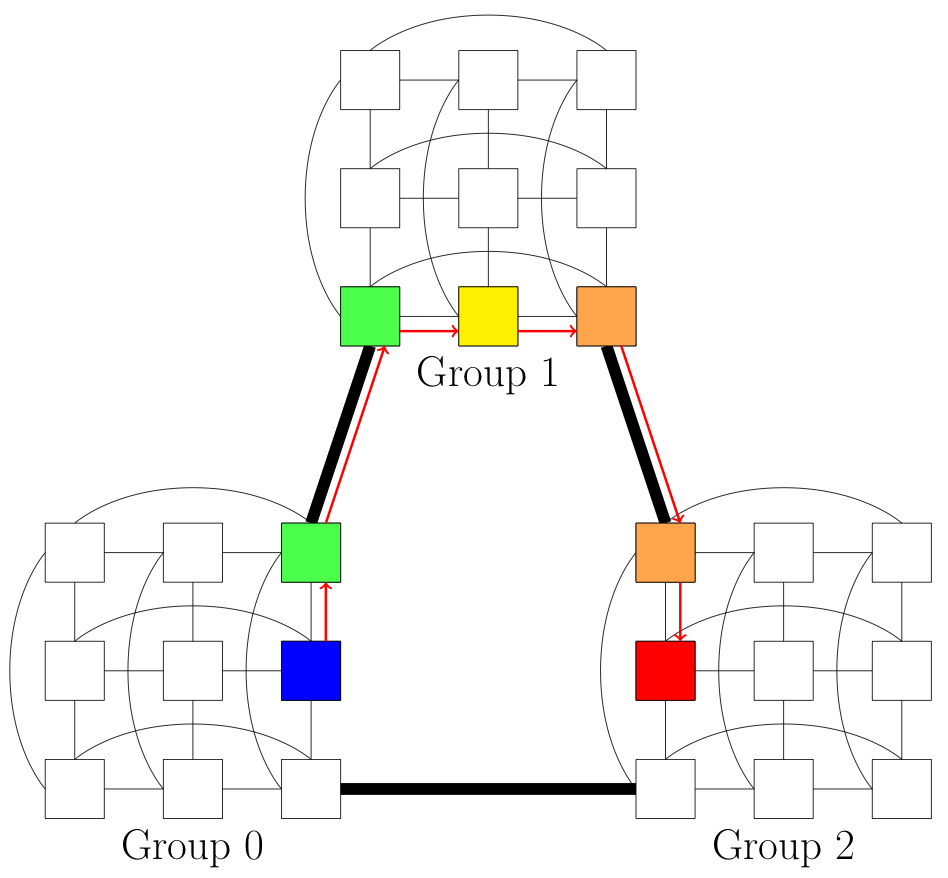
\includegraphics[width=0.7\textwidth]{figures/tikz/dragonfly/dflyvaliant.png}
\caption{Schematic of dragonfly showing Valiant route. Traveling between groups requires routing to a random intermediate node, then routing minimally to the final destination.}
\label{fig:topologies:dflyvaliantroute}
\end{figure}

To improve on minimal routing, global routing strategies are required (global routing is distinguished here from adaptive routing).  
Global essentially means ``not minimal'' and spreads packets along many different paths.
The simplest global routing strategy is Valiant routing, which falls in the global, oblivious category (Figure \ref{fig:topologies:dflyvaliantroute}).
Oblivious simply means packets are scattered randomly without measuring congestion.
In Valiant routing, each packet does the following:
\begin{itemize}
\item Pick a random intermediate node 
\item Route minimally to random node
\item Route minimally from random node to destination node
\end{itemize}
This is somewhat counterintuitive at first.
Rather than go directly to the destination node, packets go out of their way to a random node, shown in Figure \ref{fig:topologies:dflyvaliantroute} as the yellow router.
Thus, routing from the blue router in Group 0 to the red router in Group 2 first follows the minimal path (green routers) to the randomly selected yellow router in Group 1. 
From there, a second minimal path is taken through the orange routers to the final destination.
In cases with high congestion or even for large messages on a quiet network, this actually improves performance.
If a point-to-point message is composed of ten packets,
all ten packets will follow different paths to the final destination.
This essentially multiplies the maximum bandwidth by a factor of ten.
Valiant routing can be specified as

\begin{ViFile}
router = valiant
\end{ViFile}

In contrast, UGAL routing is a global, adaptive strategy, making decisions based on congestion.
Because Valiant is oblivious, it often sends too many packets to far away random nodes.
Following a Valiant path is only relevant when enough packets fill up router queues, creating congestion.
UGAL does the following steps:
\begin{itemize}
\item Start routing minimally
\item On each step, check congestion (buffer queue depth)
\item If congestion is too heavy, switch to Valiant and re-route to random intermediate node. Otherwise stay on minimal path.
\end{itemize}
UGAL packets stay on a minimal path until congestion forces them to use a Valiant strategy.
This routing can be specified as:

\begin{ViFile}
router = ugal
\end{ViFile}

